\documentclass{article}
\usepackage{graphicx} % Required for inserting images

\usepackage[margin=1in]{geometry}
\usepackage{graphicx}
\usepackage{booktabs}
\usepackage{amsmath, amssymb}
\usepackage{siunitx}            
\usepackage{caption}
\usepackage{subcaption}
\usepackage{hyperref}
\usepackage{enumitem}
\usepackage{float}             
\usepackage{xcolor}
\usepackage{adjustbox}
\usepackage{graphicx}   

\usepackage[backend=biber,style=apa]{biblatex}
\addbibresource{refs.bib}





\title{Técnicas de Agrupamiento aplicado a analizar la relación entre la salud mental, hábitos y felicidad.}
\author{Autor: Fisam Zavala}
\date{November 2025}

\begin{document}
\maketitle

%\begin{abstract}
%*PENDIENTE*
%\end{abstract}

\section{Introducción}

El análisis de agrupamiento, o \emph{clustering}, es una técnica de aprendizaje no supervisado que permite identificar patrones y estructuras subyacentes en los datos sin la necesidad de etiquetas predefinidas. Su objetivo principal es agrupar observaciones con características similares dentro del mismo conjunto, maximizando la homogeneidad interna y la heterogeneidad entre grupos.

En este trabajo se analiza un conjunto de datos sintético conformado por 3,000 observaciones y cinco variables numéricas: \textit{Sleep Hours}, \textit{Work Hours per Week}, \textit{Screen Time per Day (Hours)}, \textit{Social Interaction Score} y \textit{Happiness Score}. Dichas variables describen distintos aspectos de los hábitos de vida y el bienestar subjetivo de las personas.

El propósito de este documento es aplicar y comparar distintos métodos de agrupamiento para explorar las posibles relaciones entre los hábitos diarios y los niveles de felicidad. Para ello, se utilizarán los algoritmos \textbf{K-Means} y \textbf{DBSCAN}, complementados con el \textbf{índice de Calinski–Harabasz} como métrica para la determinación del número óptimo de clústeres en el caso de K-Means.

\section{Antecedentes}

El estudio de la felicidad y los hábitos de vida ha cobrado gran relevancia en las últimas décadas, tanto desde la psicología positiva como desde las ciencias de datos. Diversas investigaciones han demostrado que el bienestar subjetivo está estrechamente relacionado con factores cotidianos como el sueño, la actividad laboral, el tiempo frente a pantallas, la interacción social y la alimentación.

En el ámbito científico, \cite{lifestyle-ml} aplicaron técnicas de minería de datos y aprendizaje automático para identificar patrones de felicidad a partir de hábitos reportados por individuos, demostrando que la calidad del sueño y el equilibrio entre trabajo y ocio son predictores clave del bienestar. Por su parte, \cite{prospective-habits} encontraron que el optimismo y la satisfacción personal tienen efectos positivos sobre la adopción de comportamientos saludables, lo que a su vez influye en la felicidad general.

Estos antecedentes evidencian la utilidad de los métodos cuantitativos y de aprendizaje no supervisado para descubrir estructuras latentes en los datos de bienestar. Bajo este marco, el presente trabajo busca aportar una aproximación empírica mediante técnicas de agrupamiento que permitan visualizar de forma exploratoria cómo los distintos hábitos pueden asociarse con diferentes niveles de felicidad.


\section{Análisis con K-Means}

\subsection{Metodología}

El algoritmo \textit{K-Means} es uno de los métodos más utilizados en el aprendizaje no supervisado debido a su simplicidad y eficiencia. Su propósito es dividir el conjunto de datos en \(k\) grupos o clústeres, de modo que los puntos dentro de cada grupo sean lo más similares posible entre sí y lo más diferentes posible de los puntos de otros grupos.  
Matemáticamente, busca minimizar la función objetivo:

\[
J = \sum_{i=1}^{k} \sum_{x_j \in C_i} \lVert x_j - \mu_i \rVert^2
\]

donde:
\begin{itemize}
    \item \( C_i \): conjunto de observaciones asignadas al clúster \(i\),
    \item \( \mu_i \): centroide o media de los puntos en el clúster \(i\),
    \item \( \lVert x_j - \mu_i \rVert^2 \): distancia cuadrática euclidiana entre cada observación y su centroide.
\end{itemize}

El proceso iterativo de K-Means consta de los siguientes pasos:
\begin{enumerate}
    \item Seleccionar aleatoriamente \(k\) centroides iniciales.
    \item Asignar cada observación al centroide más cercano según la distancia euclidiana.
    \item Recalcular los centroides con base en las medias de cada grupo.
    \item Repetir los pasos 2 y 3 hasta que las asignaciones no cambien significativamente o se alcance la convergencia.
\end{enumerate}

\subsection{Estrategia para determinar el número óptimo de clústeres}

Una etapa fundamental en el uso de \textit{K-Means} es definir el número adecuado de clústeres (\(k\)), ya que este parámetro influye directamente en la estructura final del agrupamiento.  
Existen diversas métricas de validación interna que permiten evaluar la calidad de las particiones obtenidas. En este análisis se emplearon dos de las más utilizadas:

\begin{itemize}
    \item \textbf{Método del Codo (Elbow Method):} evalúa la \textit{inercia}, es decir, la suma de las distancias cuadráticas entre los puntos y su centroide correspondiente. Se calcula para distintos valores de \(k\), y el valor óptimo se identifica en el punto donde la disminución de la inercia deja de ser significativa, formando un “codo” en la gráfica.

    \item \textbf{Coeficiente de Silhouette:} mide la calidad de la asignación de cada observación a su clúster, comparando la distancia promedio al resto de los puntos del mismo grupo con la distancia promedio al clúster más cercano. Valores cercanos a 1 indican una buena separación entre clústeres, mientras que valores negativos sugieren una posible asignación errónea.
\end{itemize}

Ambos métodos se aplicaron para el rango \(k = 2 \text{ a } 10\), encontrándose que el punto de inflexión en el método del codo y el máximo promedio del coeficiente de Silhouette coincidieron aproximadamente en \(k = 3\), lo cual sirvió como guía para la selección inicial del número de grupos.  

\begin{figure}[H]
    \centering
    \includegraphics[width=0.8\textwidth]{figures/elbow.png}
    \caption{Método del Codo: se observa una disminución pronunciada en la inercia hasta \(k=3\), 
    punto a partir del cual la reducción se estabiliza, sugiriendo que tres clústeres son apropiados.}
    \label{fig:elbow_method}
\end{figure}

\begin{figure}[H]
    \centering
    \includegraphics[width=0.8\textwidth]{figures/silhouette.png}
    \caption{Coeficiente de Silhouette por número de clústeres. Los valores más altos 
    indican una mejor cohesión dentro de los grupos y una mayor separación entre ellos.}
    \label{fig:silhouette_scores}
\end{figure}

La siguiente tabla presenta los valores promedio de las variables numéricas 
para cada grupo identificado por el algoritmo K-Means.


\begin{table}[H]
\centering
\resizebox{\textwidth}{!}{%
  \begin{tabular}{lrrrrr}
\toprule
 & Sleep Hours & Work Hours per Week & Screen Time per Day (Hours) & Social Interaction Score & Happiness Score \\
Cluster &  &  &  &  &  \\
\midrule
0 & 6.460000 & 38.150000 & 6.140000 & 5.970000 & 3.070000 \\
1 & 6.410000 & 41.510000 & 3.210000 & 5.530000 & 5.350000 \\
2 & 6.560000 & 38.490000 & 6.150000 & 4.910000 & 7.750000 \\
\bottomrule
\end{tabular}
 
}
\caption{Resumen descriptivo de los clústeres (K-Means).}
\label{tab:kmeans_summary}
\end{table}


\section{Determinar número de grupos usando Índice de Calinski–Harabas}

En la siguiente sección se complementa este análisis mediante el uso del \textbf{índice de Calinski–Harabasz}, una métrica estadística que ofrece un criterio más formal para validar el número óptimo de clústeres.

\subsection{Metodología}

El índice de \textbf{Calinski--Harabasz (CH)} evalúa la calidad de un particionado de clústeres 
comparando la \textbf{dispersión entre clústeres} con la \textbf{dispersión dentro de los clústeres}:

\[
CH(k) = \frac{\text{Tr}(B_k)}{\text{Tr}(W_k)} \cdot \frac{n - k}{k - 1}
\]

donde:
\begin{itemize}
    \item $B_k$ es la \textbf{varianza entre grupos} (qué tan separados están los centroides),
    \item $W_k$ es la \textbf{varianza intra-grupo} (qué tan compactos son los clústeres),
    \item $n$ es el número de observaciones y $k$ el número de clústeres.
\end{itemize}

\noindent
\textbf{Interpretación:} valores más altos de $CH$ indican una \textbf{mejor separación} y \textbf{mayor compacidad} simultáneamente.  
En la práctica se calcula $CH(k)$ para varios valores de $k$ (por ejemplo, $k = 2$--$10$) y se elige el valor de $k$ con $CH$ máximo (o un máximo local estable).

\subsection{Cálculo}

En este análisis se estandarizaron las variables numéricas antes de aplicar el algoritmo, garantizando que cada una contribuyera de manera equitativa a las distancias calculadas. Se exploraron diferentes valores de \(k\) utilizando tanto el método del codo como el índice de Calinski–Harabasz, determinándose que \(k=2\) ofrecía la mejor partición en términos de equilibrio entre cohesión y separación.  

El resultado evidenció dos grupos principales: el primero concentró individuos con mayor carga laboral y niveles moderados de felicidad, mientras que el segundo incluyó a quienes trabajan menos horas semanales y presentan niveles ligeramente superiores de bienestar. Estos hallazgos se analizarán con mayor detalle en la sección de resultados.



\begin{figure}[H]
    \centering
    \includegraphics[width=0.8\textwidth]{figures/IndiceCalinski.png}
        \caption{K óptimo por Calinski–Harabasz: k = 2}
    \label{fig:elbow_method}
\end{figure}


\begin{table}[H]
\centering
\resizebox{\textwidth}{!}{%
  \begin{tabular}{lrrrrr}
\toprule
 & Sleep Hours & Work Hours per Week & Screen Time per Day (Hours) & Social Interaction Score & Happiness Score \\
Cluster &  &  &  &  &  \\
\midrule
0 & 6.550000 & 49.510000 & 4.980000 & 5.510000 & 5.530000 \\
1 & 6.410000 & 29.670000 & 5.200000 & 5.430000 & 5.260000 \\
\bottomrule
\end{tabular}
 
}
\caption{K óptimo por Calinski–Harabasz: k = 2}
\label{tab:kmeans_summary}
\end{table}


\subsection{Conclusión}

El análisis del \textbf{índice de Calinski--Harabasz (CH)} muestra que el valor máximo se alcanza en 
$k = 2$ $(CH = 537.12)$, indicando que la configuración con dos clústeres ofrece el 
\textbf{mejor equilibrio entre separación y cohesión interna}. 
A partir de este punto, el índice disminuye de forma continua, lo que sugiere que agregar más clústeres 
no mejora la estructura del agrupamiento y, por el contrario, fragmenta artificialmente los datos.

Los resultados del modelo \textbf{K-Means con $k = 2$} revelan una división clara en función de las 
\textbf{horas de trabajo por semana}, siendo esta la variable más determinante para la separación:

\begin{itemize}
    \item \textbf{Clúster 0:} personas con jornadas laborales largas ($\approx 50$ horas semanales) y niveles de felicidad ligeramente mayores.
    \item \textbf{Clúster 1:} personas con menor carga laboral ($\approx 30$ horas semanales) y felicidad algo más baja.
\end{itemize}

\noindent
En conjunto, el índice CH respalda que el modelo con dos grupos describe adecuadamente las diferencias estructurales 
del conjunto de datos, proporcionando una segmentación \textbf{interpretable y coherente} con las variables analizadas.


\section{DBSCAN Clustering}

A diferencia de \textbf{K-Means}, que requiere especificar el número de clústeres, 
el algoritmo \textbf{DBSCAN (Density-Based Spatial Clustering of Applications with Noise)} 
agrupa los datos en función de la \textbf{densidad de puntos} en el espacio. 

Su principal ventaja es que puede detectar \textbf{grupos de forma arbitraria} 
(no necesariamente esféricos) y \textbf{manejar valores atípicos (outliers)} automáticamente, 
lo que lo hace especialmente útil en conjuntos de datos reales donde la distribución no es homogénea.

\subsection{Fundamento matemático}

DBSCAN se basa en tres conceptos fundamentales:

\begin{enumerate}
    \item \textbf{Épsilon ($\varepsilon$):} radio máximo para considerar puntos vecinos.
    \item \textbf{MinPts:} número mínimo de puntos dentro del radio $\varepsilon$ para formar un clúster.
    \item \textbf{Densidad alcanzable:} un punto pertenece a un clúster si puede alcanzarse desde otro 
    punto a través de una secuencia de puntos vecinos (distancia $\leq \varepsilon$).
\end{enumerate}

Formalmente:

\begin{itemize}
    \item Si un punto $p$ tiene al menos $MinPts$ puntos dentro de una distancia $\varepsilon$, 
    se convierte en un \textbf{punto central}.
    \item Los puntos dentro de su vecindad se agregan al clúster.
    \item Los puntos que no pertenecen a ningún clúster se marcan como \textbf{ruido (outliers)}.
\end{itemize}

\subsection{Ventajas principales}

\begin{itemize}
    \item No requiere definir el número de clústeres ($k$) previamente.
    \item Detecta clústeres de forma irregular o de distinta densidad.
    \item Identifica outliers de forma natural sin necesidad de filtrarlos manualmente.
\end{itemize}

\subsection{Limitaciones}

\begin{itemize}
    \item Es sensible a la escala de los datos (por lo que se recomienda estandarizarlos).
    \item Los parámetros $\varepsilon$ y $MinPts$ requieren ajuste manual o heurístico.
    \item Puede tener un desempeño limitado en conjuntos de datos con densidad variable.
\end{itemize}

\subsection{Aplicación en el conjunto de datos}

En este análisis, se aplicó el algoritmo \textbf{DBSCAN} sobre las mismas variables numéricas utilizadas en el modelo K-Means.  
Los parámetros $\varepsilon$ y $MinPts$ fueron determinados mediante inspección visual a partir del gráfico de \textit{k-distancias}, 
seleccionando el valor de $\varepsilon$ en el punto de inflexión de la curva.  

El objetivo fue comparar la segmentación generada por DBSCAN con la de K-Means, 
evaluando si la detección de ruido y la estructura de densidad aportan una interpretación adicional sobre los hábitos y niveles de felicidad.


\begin{figure}[H]
    \centering
    \includegraphics[width=0.8\textwidth]{figures/dbscan_epsilon.png}
    \caption{Gráfico k-distancias para estimar el parámetro $\varepsilon$ en DBSCAN. 
    El punto de inflexión indica el valor adecuado de $\varepsilon$ para la segmentación.}
    \label{fig:dbscan_epsilon}
\end{figure}

\begin{figure}[H]
    \centering
    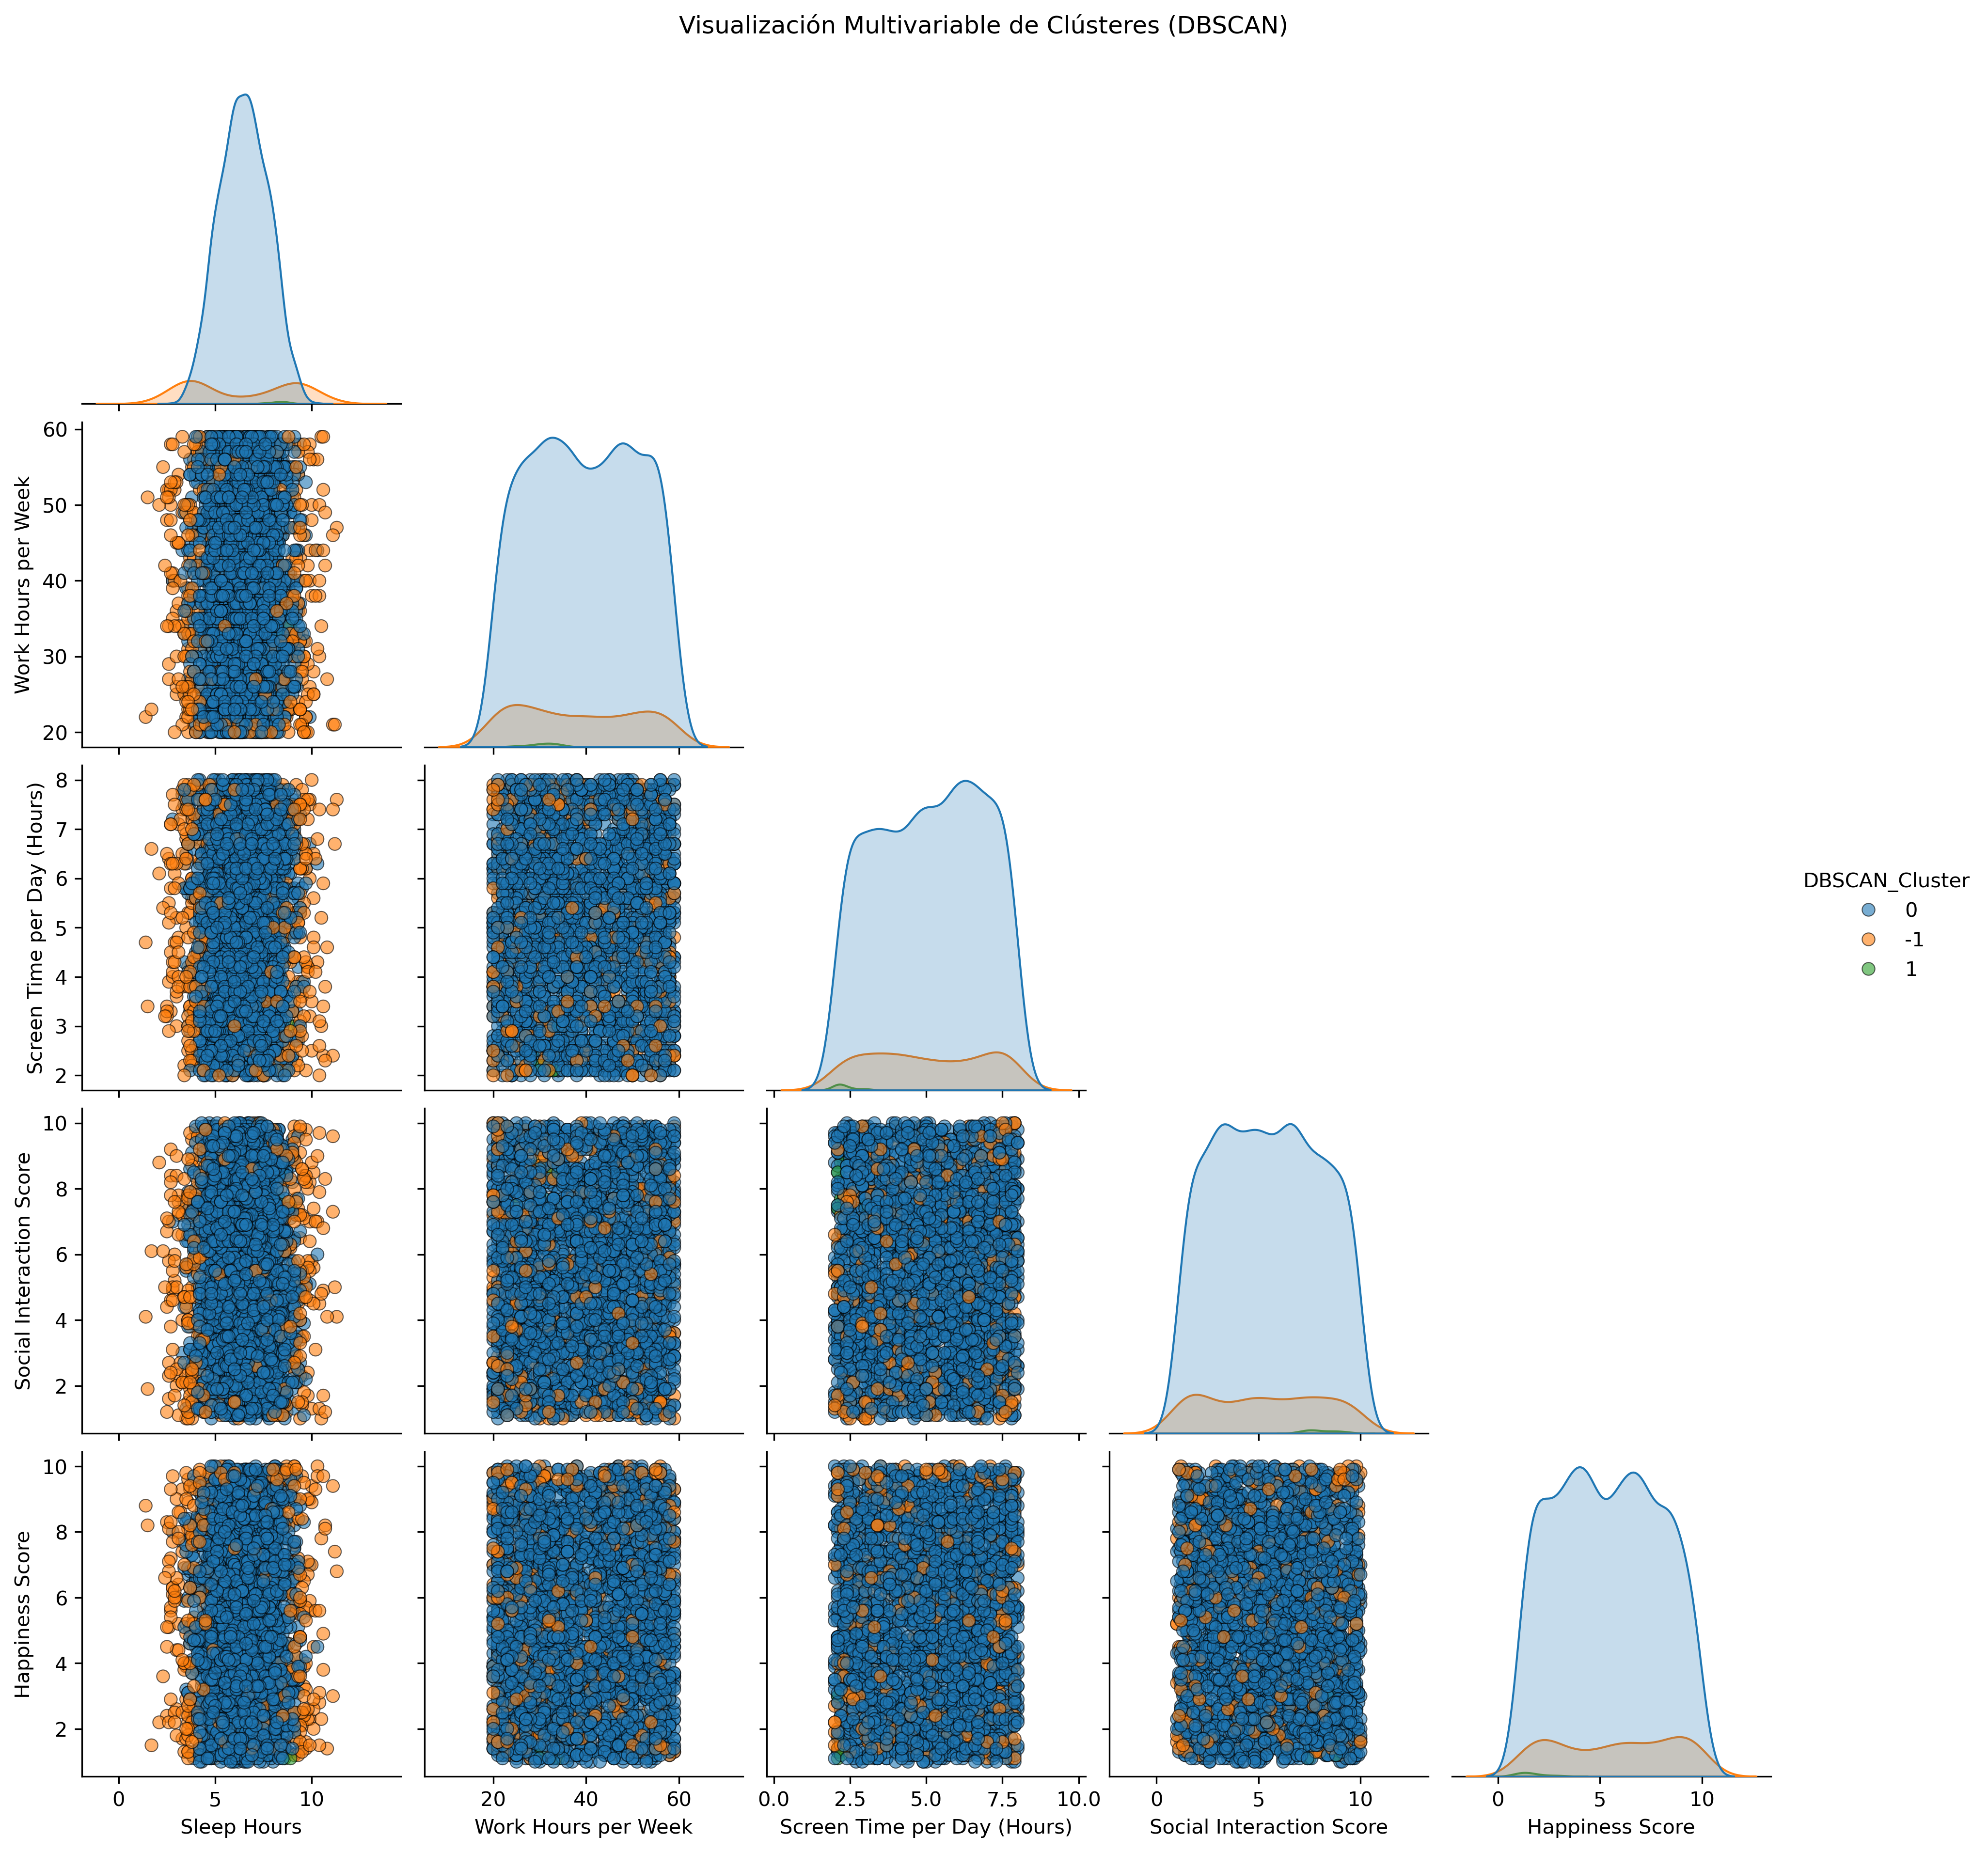
\includegraphics[width=\textwidth]{figures/dbscan_cluster.png}
    \caption{Visualización multivariable de los clústeres generados por DBSCAN. 
    Se observa la presencia de ruido (etiquetado como -1) y la distribución de los puntos según las variables analizadas.}
    \label{fig:dbscan_clusters}
\end{figure}

\begin{table}[H]
\centering
\resizebox{\textwidth}{!}{%
  \begin{tabular}{lrrrrr}
\toprule
 & Sleep Hours & Work Hours per Week & Screen Time per Day (Hours) & Social Interaction Score & Happiness Score \\
DBSCAN_Cluster &  &  &  &  &  \\
\midrule
-1 & 6.370000 & 38.390000 & 5.030000 & 5.340000 & 5.720000 \\
0 & 6.480000 & 39.630000 & 5.100000 & 5.480000 & 5.360000 \\
1 & 8.290000 & 30.710000 & 2.310000 & 8.090000 & 1.640000 \\
\bottomrule
\end{tabular}
 
}
\caption{Resumen descriptivo de los clústeres generados por el algoritmo DBSCAN. 
Se incluyen los promedios de cada variable para los clústeres 0, 1 y el ruido (-1).}
\label{tab:dbscan_summary}
\end{table}


%\section{Resultados}

\section{Discusión}

El modelo \textbf{DBSCAN} logró identificar un clúster principal y un grupo pequeño adicional, con un 
\textbf{11.7\% de ruido}. Aunque este nivel de ruido se mantiene dentro de los rangos aceptables 
(5--25\%), el resultado evidencia que la mayoría de los registros presentan una 
\textbf{densidad homogénea}, por lo que el algoritmo no logró formar más regiones densas diferenciadas.  

Este hallazgo sugiere que el \textbf{conjunto de datos no presenta agrupamientos naturales basados en densidad}, 
sino una distribución relativamente uniforme en el espacio de las variables analizadas. 
Esto contrasta con el comportamiento observado en \textbf{K-Means}, que sí logró identificar grupos 
distintos a partir de las medias de sueño, trabajo, interacción social y felicidad.

Por tanto, mientras \textbf{K-Means} consiguió segmentar a los individuos según patrones promedio 
de comportamiento, \textbf{DBSCAN} puso de manifiesto la \textbf{ausencia de regiones densas bien separadas}.  
Este resultado es metodológicamente valioso, pues evidencia que distintos algoritmos de agrupamiento 
pueden revelar estructuras complementarias (o la falta de ellas) dentro de un mismo conjunto de datos.  

En contextos donde los datos son altamente uniformes o carecen de concentraciones de densidad, 
modelos como DBSCAN tienden a producir un único clúster grande y pocos grupos pequeños. 
Sin embargo, este comportamiento no representa un fallo del método, sino una señal de que las 
\textbf{diferencias entre observaciones son más graduales que estructurales}.  

Finalmente, esta comparación entre K-Means y DBSCAN demuestra la importancia de seleccionar el método 
de agrupamiento considerando la naturaleza del fenómeno estudiado: mientras el primero se basa en 
distancias geométricas respecto a centroides, el segundo depende de densidades locales.  
Ambos, utilizados de manera complementaria, ofrecen una visión más completa sobre la estructura 
latente de los datos y sobre los posibles patrones de comportamiento asociados al bienestar.

\section{Conclusiones}

En síntesis, el análisis de agrupamiento permitió contrastar dos enfoques no supervisados con 
características complementarias. \textbf{K-Means} mostró una estructura más interpretable basada en 
promedios de variables cuantitativas, mientras que \textbf{DBSCAN} evidenció la homogeneidad del 
conjunto al no detectar regiones densas bien definidas.  

Estos resultados reflejan que el fenómeno analizado, la relación entre hábitos y felicidad,
no presenta divisiones tajantes entre grupos de individuos, sino gradientes continuos de comportamiento.  
Así, más que segmentaciones estrictas, los hallazgos sugieren que el bienestar puede explicarse mejor 
como una combinación progresiva de factores personales y sociales.  

Desde una perspectiva metodológica, el trabajo demuestra la utilidad de combinar distintos 
algoritmos de aprendizaje no supervisado para obtener una visión más robusta de los datos, 
evaluando tanto su estructura geométrica como su distribución de densidades.  


\renewcommand{\refname}{Referencias}
\begin{thebibliography}{9}

\bibitem{JPMS2023}
Khan, A., & Ali, M. (2023). 
\textit{Can Lifestyle Habits Predict Happiness? An Exploratory Machine Learning Study Using a Visual Data Mining Platform.} 
\textit{Journal of Pakistan Medical Students (JPMS).} 
Recuperado de \url{https://jpmsonline.com/article/can-lifestyle-habits-predict-happiness-an-exploratory-machine-learning-study-using-a-visual-data-mining-platform-755}

\bibitem{BMC2019}
Steptoe, A., & Wardle, J. (2019). 
\textit{Prospective Associations of Happiness and Optimism with Lifestyle Habits and Health Outcomes.} 
\textit{BMC Public Health.} 
Recuperado de \url{https://pmc.ncbi.nlm.nih.gov/articles/PMC6697576/}

\bibitem{Preventive2021}
Schnettler, B., & Miranda-Zapata, E. (2021). 
\textit{Subjective Well-being Predicts Health Behavior in a 9-Years Follow-up.} 
\textit{Preventive Medicine Reports.} 
Recuperado de \url{https://www.sciencedirect.com/science/article/pii/S2211335521003260}

\bibitem{Nature2025}
Park, J., & Kim, S. (2025). 
\textit{Graphical Model Analysis of Subjective Well-being and Various Factors.} 
\textit{Scientific Reports (Nature Portfolio).} 
Recuperado de \url{https://www.nature.com/articles/s41598-025-98064-2}

\bibitem{IJQW2023}
Thompson, C., & Lee, Y. (2023). 
\textit{The Relationship Between Subjective Well-being and Food: A Qualitative Study of Children’s Perspectives.} 
\textit{International Journal of Qualitative Studies on Health and Well-being.} 
Recuperado de \url{https://www.tandfonline.com/doi/full/10.1080/17482631.2023.2189218}

\end{thebibliography}

\end{document}
